 \documentclass[12pt]{article}
\usepackage[a4paper, margin=.30in]{geometry}

\usepackage{array}
\usepackage{graphicx, subfig, wrapfig, fancyhdr, lastpage,makecell }
\newcommand\headerMe[2]{\noindent{}#1\hfill#2}
\usepackage[mathscr]{euscript}



\pagestyle{fancy}
\fancyhf{}

\rfoot{\em{Page \thepage \hspace{1pt} / \pageref{LastPage}}}
\begin{document}

\headerMe{Royaume du Maroc}{année scolaire \emph{2024-2025}}\\
\headerMe{Ministère de l'Éducation nationale, }{  Professeur :\emph{Zakaria Haouzan}}\\
\headerMe{du Préscolaire et des Sports}{Établissement : \emph{Lycée SKHOR qualifiant}}\\

\begin{center}

	Devoir  N°2 \\
	Filière Tronc Commun Scientifique\\
	Durée 2h00
	\\
	\hrulefill
	\Large{Chimie 7pts - 36min}
	\hrulefill\\

	%\emph{Les Trois parties sont indépendantes}
\end{center}
%end Headerss------------------------


\section*{Partie1: Le modèle de l'atome  \dotfill (3,5pts) }
%\begin{wrapfigure}[5]{r}{0.36\textwidth}
%\vspace{-1.8cm}
%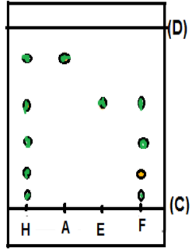
\includegraphics[width=0.36\textwidth]{./img/CCM.png}
%\end{wrapfigure}
L’atome de sodium Na contient 23 nucléons et 11
électrons.

Données : $m_p = m_n = 1,7.10^{-27}kg$ , $1pm = 10^{-12}m$ , $1m^3  =10^6 cm^3$

\begin{enumerate}

	\item Déterminer le numéro atomique de cet
	      atome.\dotfill(0,5pt)
	\item  Donner le symbole de cet atome.\dotfill(0,5pt)
	\item  Calculer la masse de cet atome.\dotfill(0,5pt)
	\item Calculer le nombre des atomes de sodium
	      contenus dans un échantillon de sodium
	      de masse $m=23,20g$.\dotfill(0,5pts)
	\item  Le rayon de l’atome de sodium est
	      $r=190pm$, calculer son volume exprimé en $m^3$ et $cm^3$.\dotfill(0,5pt)
	\item  Donner la formule électronique de cet
	      atome .la couche externe est-elle saturée
	      justifier votre réponse.\dotfill(1pt)
\end{enumerate}

\section*{Partie 2: formule électronique d'un atome \dotfill(3,5pts)}
La formule électronique d'un atome est: $(K)^2(L)^8(M)^7$.

\begin{enumerate}
	\item Quel est le nom de la couche externe de cet atome?\dotfill(0,5pt)

	\item Combien d'électrons externes cet atome possède-t-il?\dotfill(0,5pt)

	\item Donner le symbole de son noyau sous la forme ${^{A}_{Z}X}$, sachant que l'élément correspondant est le chlore et que son noyau comporte 18 neutrons.\dotfill(0,5pt)

	\item Donner la composition de cet atome.\dotfill(0,5pt)

	\item Quel est la masse de cet atome?\dotfill(0,5pt) \\
	      Données :
	      \begin{itemize}
		      \item Masse du proton = masse du neutron = $1,67 \times 10^{-27}$ kg
		      \item Masse de l'électron = $9,10 \times 10^{-31}$ kg
	      \end{itemize}

	\item Quel ion cet atome est-il susceptible de donner et pourquoi? Enoncer la loi utilisée et donner la structure électronique de cet ion.\dotfill(1pt)
\end{enumerate}

%__________________Chimie ______________________-
%%%%%%%+_+_+_+_+_+_+_+_+_Partie1

\newpage
%_____________________________________PHYSIque Partie 22222____________________________________________________________________________
\begin{center}
	%\vspace{2cm}
	\hrulefill
	\Large{Physique 13pts - 84min}
	\hrulefill\\
	\emph{Les  parties sont indépendantes}
\end{center}
%end Headerss------------------------
\section*{Exercice 1: Le mouvement \dotfill(13pts) }
\section*{Partie 1 :Le Mouvement rectiligne uniforme \dotfill(4 pts)}
On considère deux voitures A et B en mouvement rectiligne uniforme sur une partie d’une autoroute avec les vitesses respectivement $V_A=72Km.h^{-1}$ et $V_B=108Km.h^{-1}$.
%\begin{wrapfigure}{r}{0.36\textwidth}
\begin{center}
	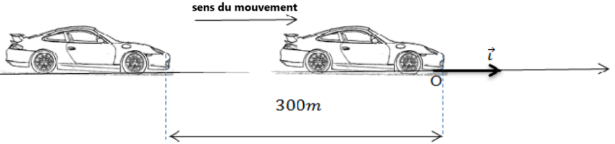
\includegraphics[width=0.56\textwidth]{./img/ex1.png}
\end{center}
%\end{wrapfigure}


A l’instant $t=0$ la voiture B est à $300m$ derrière la voiture A.
On choisit la position O, la position de la voiture A à l’instant $t=0$ ; comme origine des abscisses et des dates.

\begin{enumerate}
	\item  Convertir la valeur de $V_A$ et $V_B$ en $m.s^{-1}$.\dotfill(1pt)
	\item Ecrire l’équation horaire du mouvement de chacune des voitures (A) et (B) sur l’axe $(Ox)$.\dotfill(1pt)
	\item  Déterminer l’instant $t$ et l’abscisse $x$ du doublage de la voiture (A) par la voiture (B).\dotfill(2pt)
\end{enumerate}

\section*{Partie 2: Le Mouvement de l'autoporteur \dotfill(9 pts)}
Un mobile autoporteur S, de masse m, glisse sur un plan horizontal.

On enregistre les positions occupées par un point A du mobile à intervalle de temps $\tau = 40 ms$. On obtient l’enregistrement suivant :
\begin{center}
	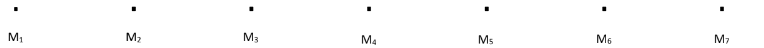
\includegraphics[width=0.8\textwidth]{./img/ex2.png}
\end{center}

\begin{enumerate}

	\item Calculer la vitesse instantanée $V_2$ et $V_4$ respectivement en $M_2$ et $M_4$.\dotfill(1pt)
	\item Déterminer la nature du mouvement du mobile, justifier.\dotfill(1pt)
	\item Déterminer les caractéristiques des vecteurs vitesses instantanées du mobile aux positions $M_1$ et $M_4$.\dotfill(1pt)


	\item Représentez $V_2$ en utilisant l'échelle de votre choix.\dotfill(1pt)
	\item On considère $M_2$ l’origine des abscisses et $M_1$ l’origine des dates, déterminer l’équation horaire du mouvement.\dotfill(1pt)
	\item Déterminer le moment de passage d'autoporteur par la position $M_4$.\dotfill(1pt)

	\item Calculer la distance parcourus par l’autoporteur (S) durant 3s.\dotfill(1pt)
	\item Un disque de rayon $R = 8cm$ tourne avec une vitesse de $45$ tours par min.
	      \begin{enumerate}
		      \item  Déterminer la nature du mouvement  \dotfill(1pt)

		      \item Calculer la fréquence du mouvement et déduire sa période.\dotfill(1pt)

	      \end{enumerate}
\end{enumerate}



\end{document}
